% ------------------------------------------------------------------------
% ------------------------------------------------------------------------
% ------------------------------------------------------------------------
%                                Capítulo 3
% ------------------------------------------------------------------------
% ------------------------------------------------------------------------
% ------------------------------------------------------------------------

\chapter{Metodología}

El enfoque de red neuronal profunda propuesto para la clasificación de objetos desde medidas cuadráticas codificadas incluye tres etapas principales: (i) capa de adquisición, (ii) enfoque de inicialización, (iii) y red de clasificación. La Figura \ref{fig:esquema_entrenamiento} ilustra el esquema de red neuronal profunda propuesto. Primero, una capa de adquisición simula el proceso de medición \eqref{eq:phase_retrieval_problem}, donde la capa realiza un modelo de propagación del campo óptico. Luego, un procedimiento de inicialización aproxima el campo óptico $\mathbf{x}$, finalmente, la red de clasificación infiere la clase correspondiente a cada medida cuadrática codificada.


\begin{figure*}[!h]
    \centering
    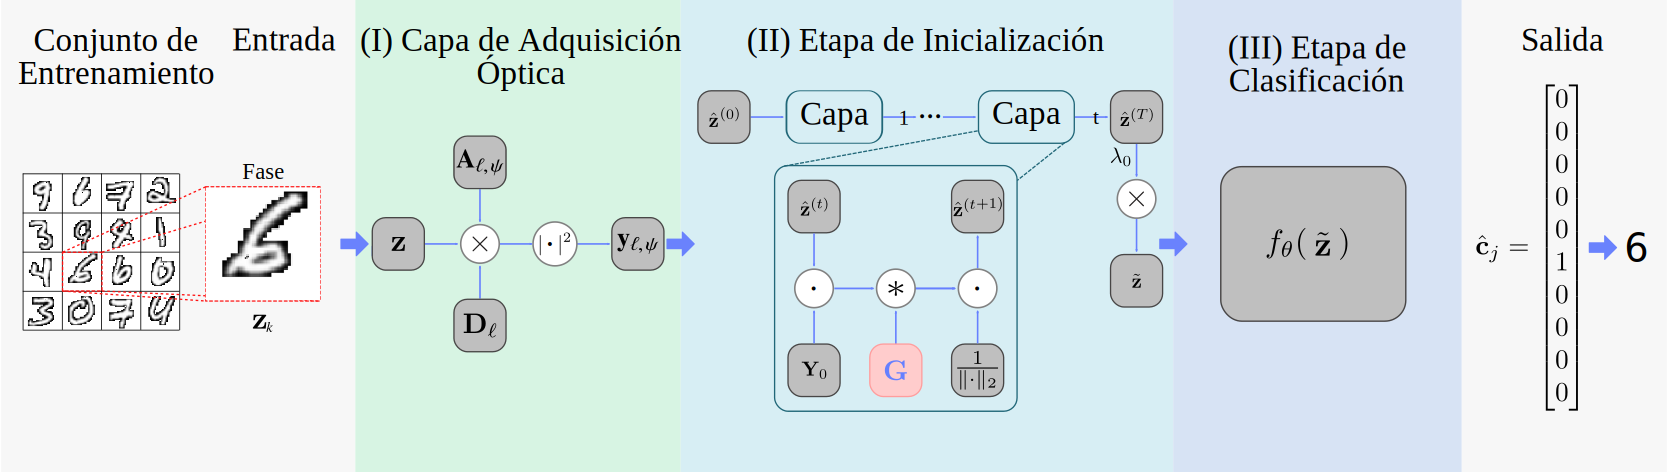
\includegraphics[width=\linewidth]{images/esquema_entrenamiento.pdf}
    \caption{\textcolor{red}{Esquema de red neuronal profunda de tres etapas propuesto para la clasificación de objetos desde medidas cuadráticas codificadas. HAY QUE CAMBIAR LA IMAGEN, ESTA NO TIENE LAS 3 ETAPAS. Posiblemente modificar la figura de la ampliación del artículo para que en vez de las unets tenga la arquitectura de clasificación.}}
    \label{fig:esquema_entrenamiento}
\end{figure*}


\section{Bloque de inicialización}

Para realizar la etapa de inicialización del campo óptico, este trabajo toma ventaja del hecho de que la matriz de adquisición $\mathbf{A}_\ell$ es conocida, por lo tanto, se crea un mapeo $\mathcal{B}(\cdot)$ que pasa de las medidas $\mathbf{y}_\ell$ a una aproximación más cercana del campo óptico $\mathbf{x}$, dada por el desenvolvimiento de un algoritmo tradicional y un conjunto de capas convolucionales, de tal forma que $\hat{\mathbf{x}}=\mathcal{B}(\mathbf{y}_\ell)$. 

% El primer enfoque usa el operador de propagación hacia atrás inverso $\mathcal{P}_\ell:\mathbb{C}^n\rightarrow \mathbb{C}^n$ del campo óptico para aproximar$\hat{\mathbf{x}}$  \myfootcite{katkovnik2017computational}, que viene dado por

% \begin{equation}
%     \hat{\mathbf{x}}= \frac{1}{L}\sum_{\ell=1}^{ L} \mathcal{P}_\ell(\mathbf{y}_\ell).
%     \label{eq:back_propagation}
% \end{equation}

Más concretamente este enfoque aplica un desenvolvimiento del algoritmo de inicialización de filtrado espectral (FSI\myfootcite{jerez2020fast}, por sus siglas en inglés). Esta inicialización se basa en un método de iteración de potencia para aproximar el campo óptico desde patrones codificados de difracción, el cual se resume en el Algoritmo \ref{alg_1}.

\begin{algorithm}[!h]
    %\scriptsize
    \caption{Algoritmo FSI}\label{fsi_algo}
    \textbf{Entrada:} Matriz de sensado y medidas adquiridas $\{(\mathbf{A}_\ell;\mathbf{y}_\ell)\}_{\ell=1}^L$, máximo número de iteraciones $T$ y el filtro pasa bajas $ \mathbf{G}$.\newline
    \textbf{Salida:} $\hat{\mathbf{x}}$.
    \begin{algorithmic}[1]
        \State{$\tilde{\mathbf{x}}^{(0)} \leftarrow$ Aleatoriamente escogido}
        \State{ $ {\nu_\Xi}_\ell \left( \left( \mathbf{y}_\ell \right)_{i} \right) = 
                \begin{cases}
                1 & i \in \Xi_\ell \\
                0 & \text{De otra forma } \\
                \end{cases},1\leq i\leq n $
                }
        \State{ $ \tilde{\mathbf{y}}_\ell = \left[ {\nu_\Xi}_\ell \left( \left( \mathbf{y}_\ell \right)_1 \right),\cdots,{\nu_\Xi}_\ell \left( \left( \mathbf{y}_\ell \right)_n \right) \right]^T$ \Comment{Truncamiento por umbral} }
        \For{$t = 0: T-1$ }
        \State{$\tilde{\mathbf{x}}^{(t+1)} \leftarrow \sum_{\ell=1}^{L}\mathcal{P}_\ell\left(  \tilde{\mathbf{y}}_\ell \odot \mathbf{A}_\ell  \tilde{\mathbf{x}}^{(t)} \right) $ }
        \State{$\tilde{\mathbf{x}}^{(t+1)} \leftarrow {\mathbf{G}} * \tilde{\mathbf{x}}^{(t)}$\Comment{Operador de convolución}}
        
       \State{$\tilde{\mathbf{x}}^{(t+1)} \leftarrow \frac{\tilde{\mathbf{x}}^{(t+1)}}{{\Vert \tilde{\mathbf{x}}^{(t+1)} \Vert}_2 }$	\Comment{Normalización}}
        \EndFor
        \State{$\hat{\mathbf{x}}^{(T)} =  \tilde{\mathbf{x}}^{(T)} \sqrt{\frac{\sum_{\ell=1}^{L} \Vert\mathbf{y}_\ell \Vert_{2}^2 }{nL} } $\Comment{Escalado}}
    \end{algorithmic}
    \label{alg_1}
\end{algorithm}

El algoritmo FSI crea el conjunto de índices $\Xi_\ell$ correspondientes a los valores más grandes de $\{(\mathbf{y}_\ell)_{i}/\vert \vert\mathbf{a}_{\ell,i}\vert \vert_2\}$, donde $\mathbf{a}_{\ell,i}\in\mathbb{C}^{n}$ representan las filas de $\mathbf{A}_\ell$. Adicionalmente, el algoritmo incluye un filtro $\mathbf{G}$, el cual fue implementado como una capa convolucional, de tal manera que cada iteración del algoritmo FSI se aplica un filtrado que promueve mejoría en la aproximación, por lo tanto una mejora en la clasificación. 
\section{Bloque de clasificación}

En este trabajo se hizo uso de la arquitectura de red de clasificación MobilNetV2 \myfootcite{sandler2018mobilenetv2} como la red de clasificación $f_\theta(\cdot)$. La Figura. \ref{fig:mobilnetv2} ilustra la arquitectura usada. La entrada pasa a través de una capa convolucional con 32 canales, luego, 7 bloques residuales de cuello de botella reducen la dimensión de los datos y aumentan el número de canales para extraer las características. Finalmente, la capa convolucional resultante toma una entrada con forma de $1\times1\times1280$ para aplicar filtros convolucionales de $1\times1$ con el número de canales igual al numero de clases en el dataset.

\begin{figure}[!h]
    \centering
    \includegraphics[width=1\linewidth]{images/MobilNet.pdf}
    \caption{Arquitectura de red MobilnetV2.}
    \label{fig:mobilnetv2}
\end{figure}

Para entrenar los pesos $\theta$ de la red de clasificación $f_\theta(\cdot)$, se puede usar el siguiente problema de optimización

\begin{equation}
    \mathbf{\theta}^* \in  \argmin_{\mathbf{\theta}} \frac{1}{J}\sum_{j = 1}^{J} \mathcal{L}\left( c^{(j)}, f_{\mathbf{\theta}}\left(\mathcal{B}(\mathbf{y}_{\ell}^{(j)})\right)\right).
    \label{eq:dl_optimization}
\end{equation}

Este problema minimiza la función pérdida usualmente llamada entropía categórica cruzada $\mathcal{L}(\cdot, \cdot)$ entre las etiquetas del dataset $c^{(j)}$, y las clases predichas $\hat{c}^{(j)} = f_\theta(\mathcal{B}(\mathbf{y}_\ell^{(j)}))$, donde $J$ es el número total de medidas y $\mathbf{y}_\ell^{(j)}$ es la medida cuadrática codificada al  j-ésimo ejemplo.
